\documentclass[11pt, a4paper]{article}
\usepackage[a4paper, margin=2.5cm]{geometry}
\usepackage[slovene]{babel}
\usepackage{enumitem}
\usepackage{float}
\usepackage{booktabs}
\usepackage{parskip}
\usepackage[hidelinks]{hyperref}
\usepackage{graphicx}

\begin{document}
\renewcommand*\contentsname{Kazalo}
\renewcommand*\tablename{Tabela}
\renewcommand*\figurename{Slika}

\begin{titlepage}
    \centering
    \vspace*{2cm}
    {\Large Univerza v Mariboru \\
    Fakulteta za elektrotehniko, računalništvo in informatiko \par}
    \vspace{0.5cm}

    \vspace{5cm}
    {\Huge \textbf{Nexus Orbital} \par}

    \vspace{11cm}
    \begin{flushleft}
        \large
        \textbf{Člani skupine:} \\
        Marko Štuhec \\
        Nik-Štefan Vodušek
    \end{flushleft}

    \vfill
    {\large Maribor, november 2026 \par}
\end{titlepage}

\tableofcontents

\section{Uvod}

Projekt \textbf{Nexus Orbital} predstavlja zasnovo spletne platforme za podjetje, ki razvija in upravlja avtonomne satelite v zemeljski orbiti. Glavni problem, ki ga rešujemo, je nepreglednost in razpršenost tehničnih podatkov v vesoljski industriji. Potencialni poslovni partnerji in raziskovalne ustanove morajo pri iskanju zmogljivosti za izstrelitev lastnega tovora pogosto prebirati obsežne dokumente PDF in pošiljati splošna povpraševanja, preden sploh ugotovijo, katera satelitska platforma ustreza njihovim potrebam.

Namen spletne rešitve Nexus Orbital je na enem mestu združiti predstavitev ključnih tehnologij, interaktivni pregled satelitske flote, časovnico preteklih in načrtovanih misij ter enostaven obrazec za rezervacijo prostora za tovor. V tem dokumentu analiziramo tri obstoječe spletne rešitve s področja komercialnih satelitskih storitev in izstrelitev, da bi prepoznali njihove dobre prakse ter pomanjkljivosti, ki jih lahko z našo rešitvijo izboljšamo.

\section{Analiza obstoječih rešitev}

\subsection{SpaceX Rideshare}

\textbf{Kratek opis:} \\
SpaceX Rideshare je spletna platforma ameriškega vesoljskega podjetja SpaceX, ki komercialnim naročnikom in raziskovalnim organizacijam omogoča rezervacijo mesta za manjše satelite na skupnih izstrelitvah rakete Falcon 9 v nizkozemeljsko ali sončno sinhrono orbito \cite{spacex}. Stran je zasnovana kot neposredno orodje za hiter izračun cene in oddajo spletnega naročila za prevoz tovora v orbito.

\textbf{Ključne funkcionalnosti:}
\begin{itemize}
    \item \textbf{Spletni konfigurator tovora:} Uporabnik izbere vrsto orbite, želeno časovno okno izstrelitve in maso tovora, sistem pa samodejno izračuna okvirno ceno storitve.
    \item \textbf{Pregled standardnih priključnih plošč:} Prikaz različnih dimenzij in nosilnosti priključnih vmesnikov.
    \item \textbf{Spletna rezervacija in tehnična dokumentacija:} Možnost neposrednega začetka naročila preko spletnega obrazca ter dostop do priročnika za integracijo tovora.
\end{itemize}

\textbf{Prednosti in slabosti:}
\begin{itemize}
    \item \textbf{Prednosti:} Zelo visoka cenovna preglednost že na prvi strani, enostaven in hiter interaktivni konfigurator ter sodoben temen vmesnik z jasno vizualno hierarhijo.
    \item \textbf{Slabosti:} Platforma je osredotočena izključno na sam prevoz v orbito in ne omogoča primerjave različnih vrst satelitskih nosilcev ali podrobnega pregleda prihodnjih misij, podrobnejši tehnični pogoji pa so skriti v obsežni datoteki PDF.
\end{itemize}

\begin{figure}[H]
    \centering
    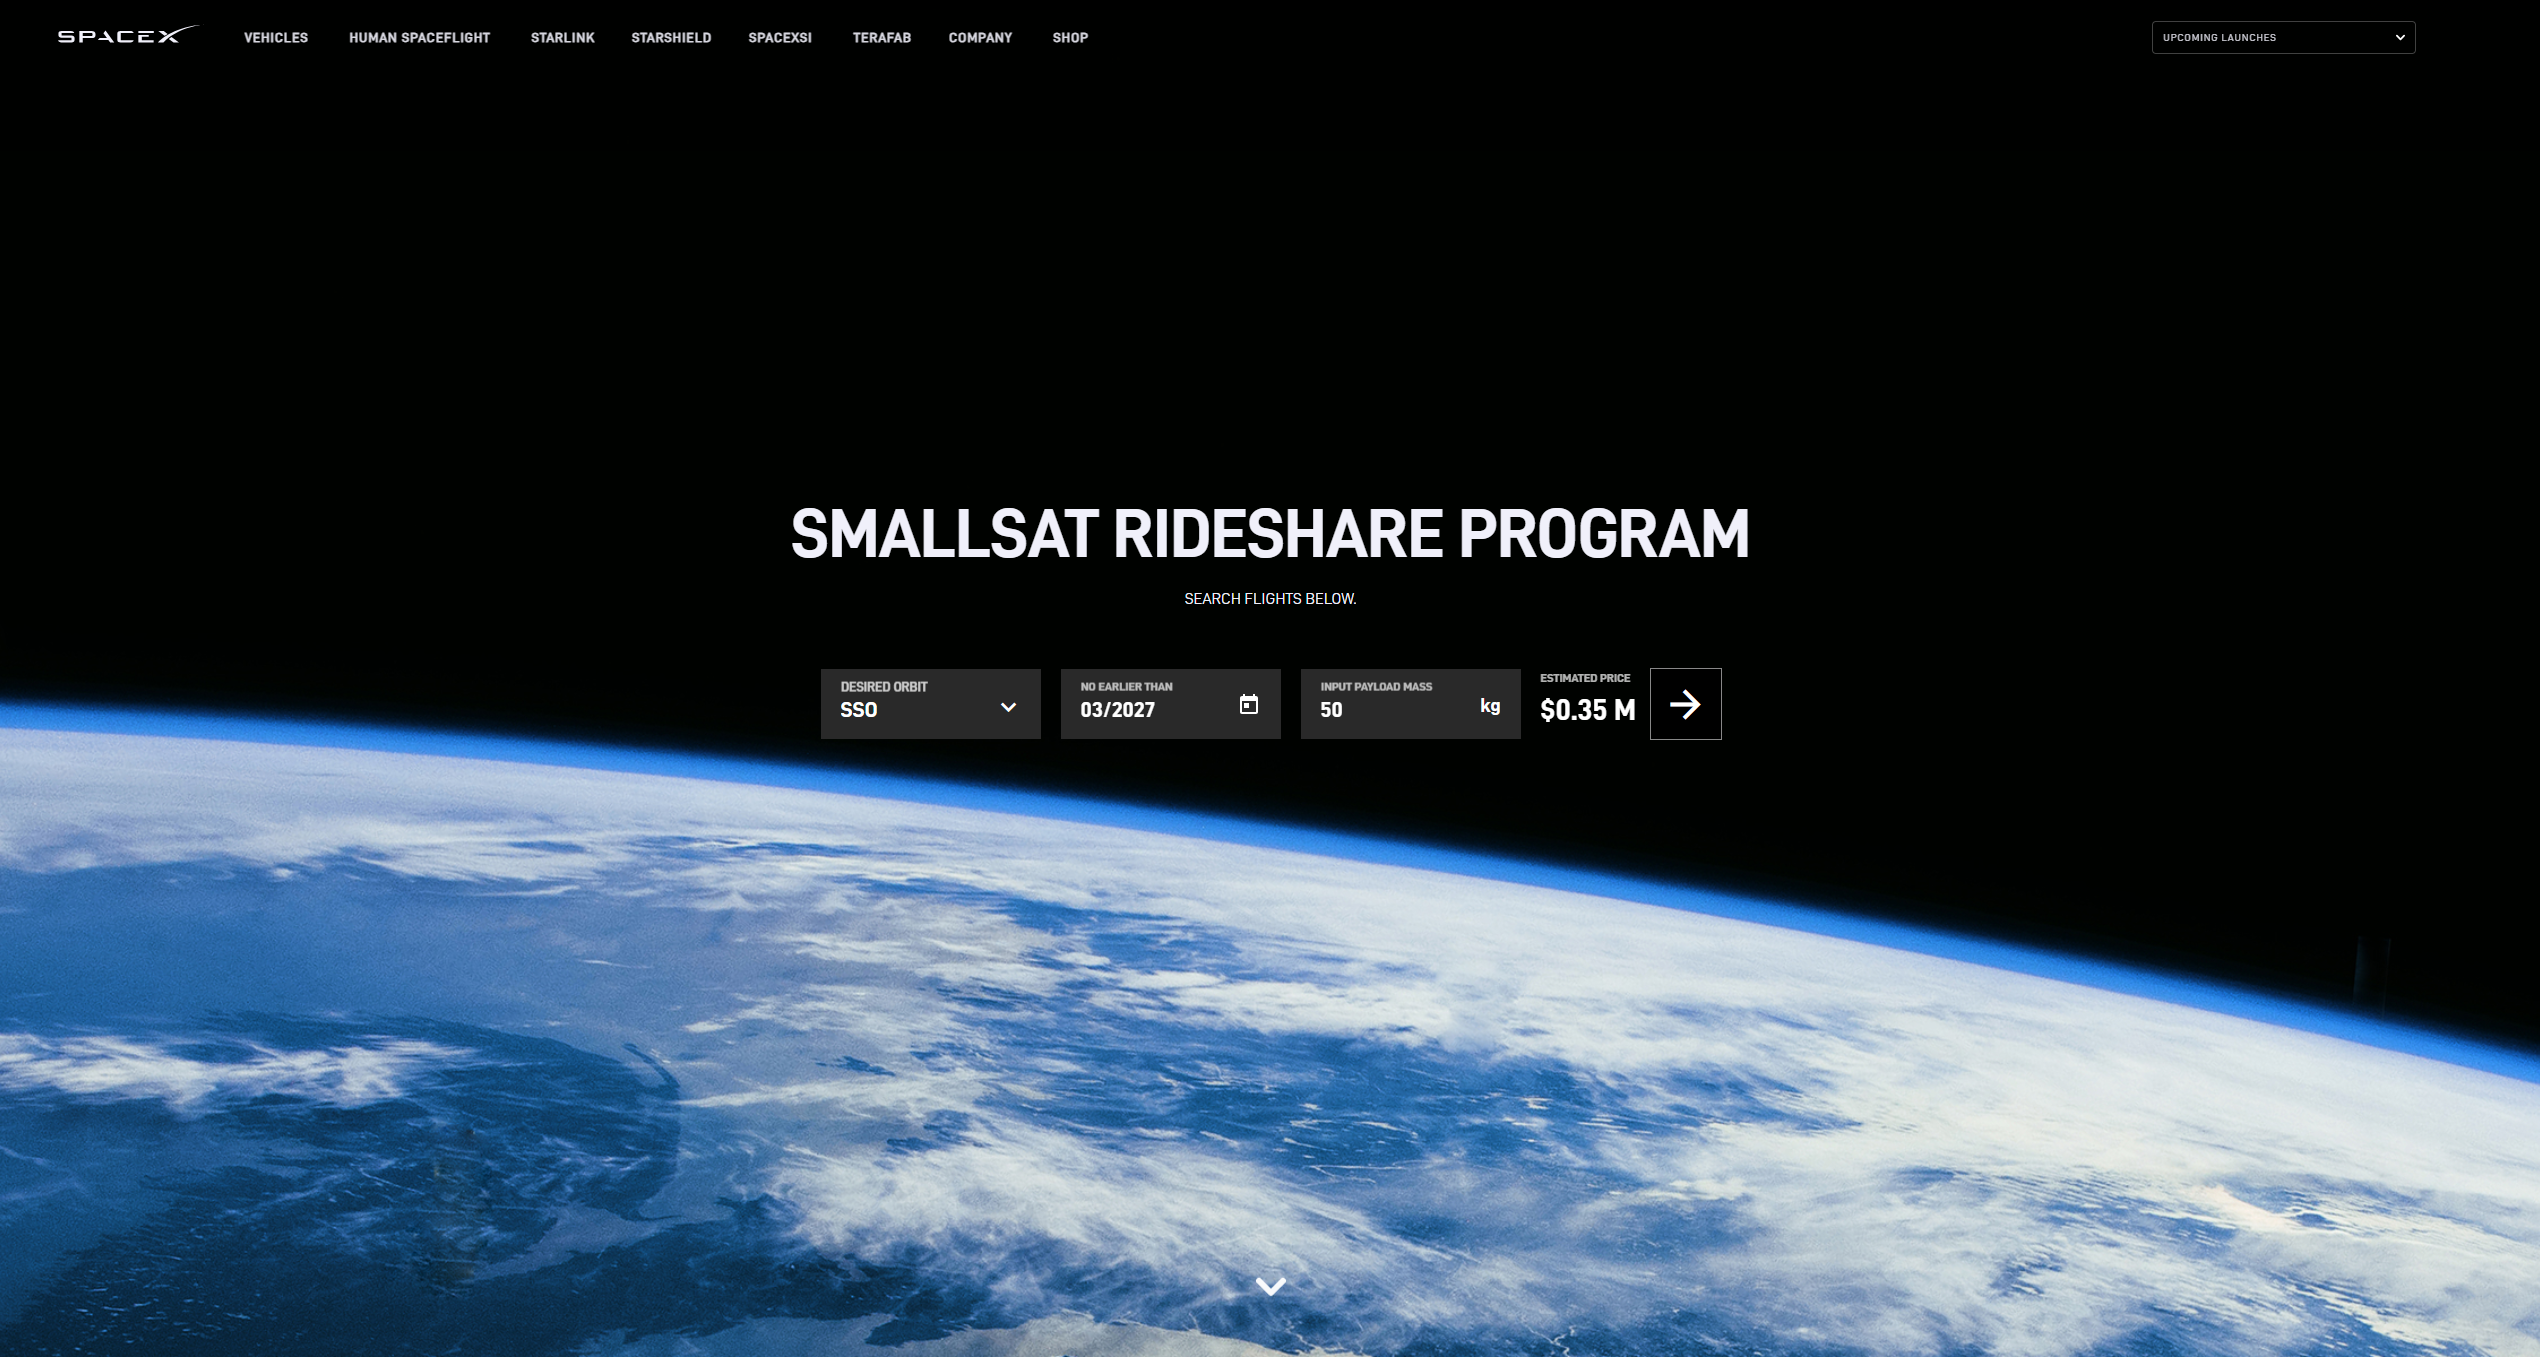
\includegraphics[width=1\linewidth]{SpaceX.png}
    \caption{Konfigurator tovora in pregled cen na platformi SpaceX Rideshare \cite{spacex}.}
    \label{fig:spacex}
\end{figure}

\subsection{Rocket Lab -- Spacecraft}

\textbf{Kratek opis:} \\
Spletna predstavitev satelitskih sistemov podjetja Rocket Lab predstavlja družino modularnih satelitskih platform (vključno s platformami Photon), namenjenih misijam v nizki zemeljski orbiti, geostacionarni orbiti ter globokem vesolju \cite{rocketlab}. Rešitev je namenjena poslovnim in institucionalnim naročnikom, ki potrebujejo celovito satelitsko platformo za svoj merilni ali komunikacijski tovor.

\textbf{Ključne funkcionalnosti:}
\begin{itemize}
    \item \textbf{Razdelitev satelitskih platform po namenu:} Prikaz različnih konfiguracij plovil glede na zahtevnost in profil vesoljske misije.
    \item \textbf{Predstavitev ključnih podsistemov:} Opis pogonskega sistema, avionike, komunikacijske opreme in napajanja posamezne platforme.
    \item \textbf{Prikaz preteklih misij in kontaktni obrazec:} Izpostavitev že uspešno izvedenih odprav za krepitev zaupanja ter obrazec za vzpostavitev stika s prodajno ekipo.
\end{itemize}

\textbf{Prednosti in slabosti:}
\begin{itemize}
    \item \textbf{Prednosti:} Jasna strukturiranost ponudbe glede na tip misije, močan poudarek na preverjenosti opreme v vesolju ter kakovostna kombinacija vizualnega materiala in tehničnih povzetkov.
    \item \textbf{Slabosti:} Tehnične specifikacije posameznih platform so razdeljene na več ločenih podstrani in datotek PDF, zato obiskovalec nima možnosti hitre primerjave parametrov v enem pogledu.
\end{itemize}

\begin{figure}[H]
    \centering
    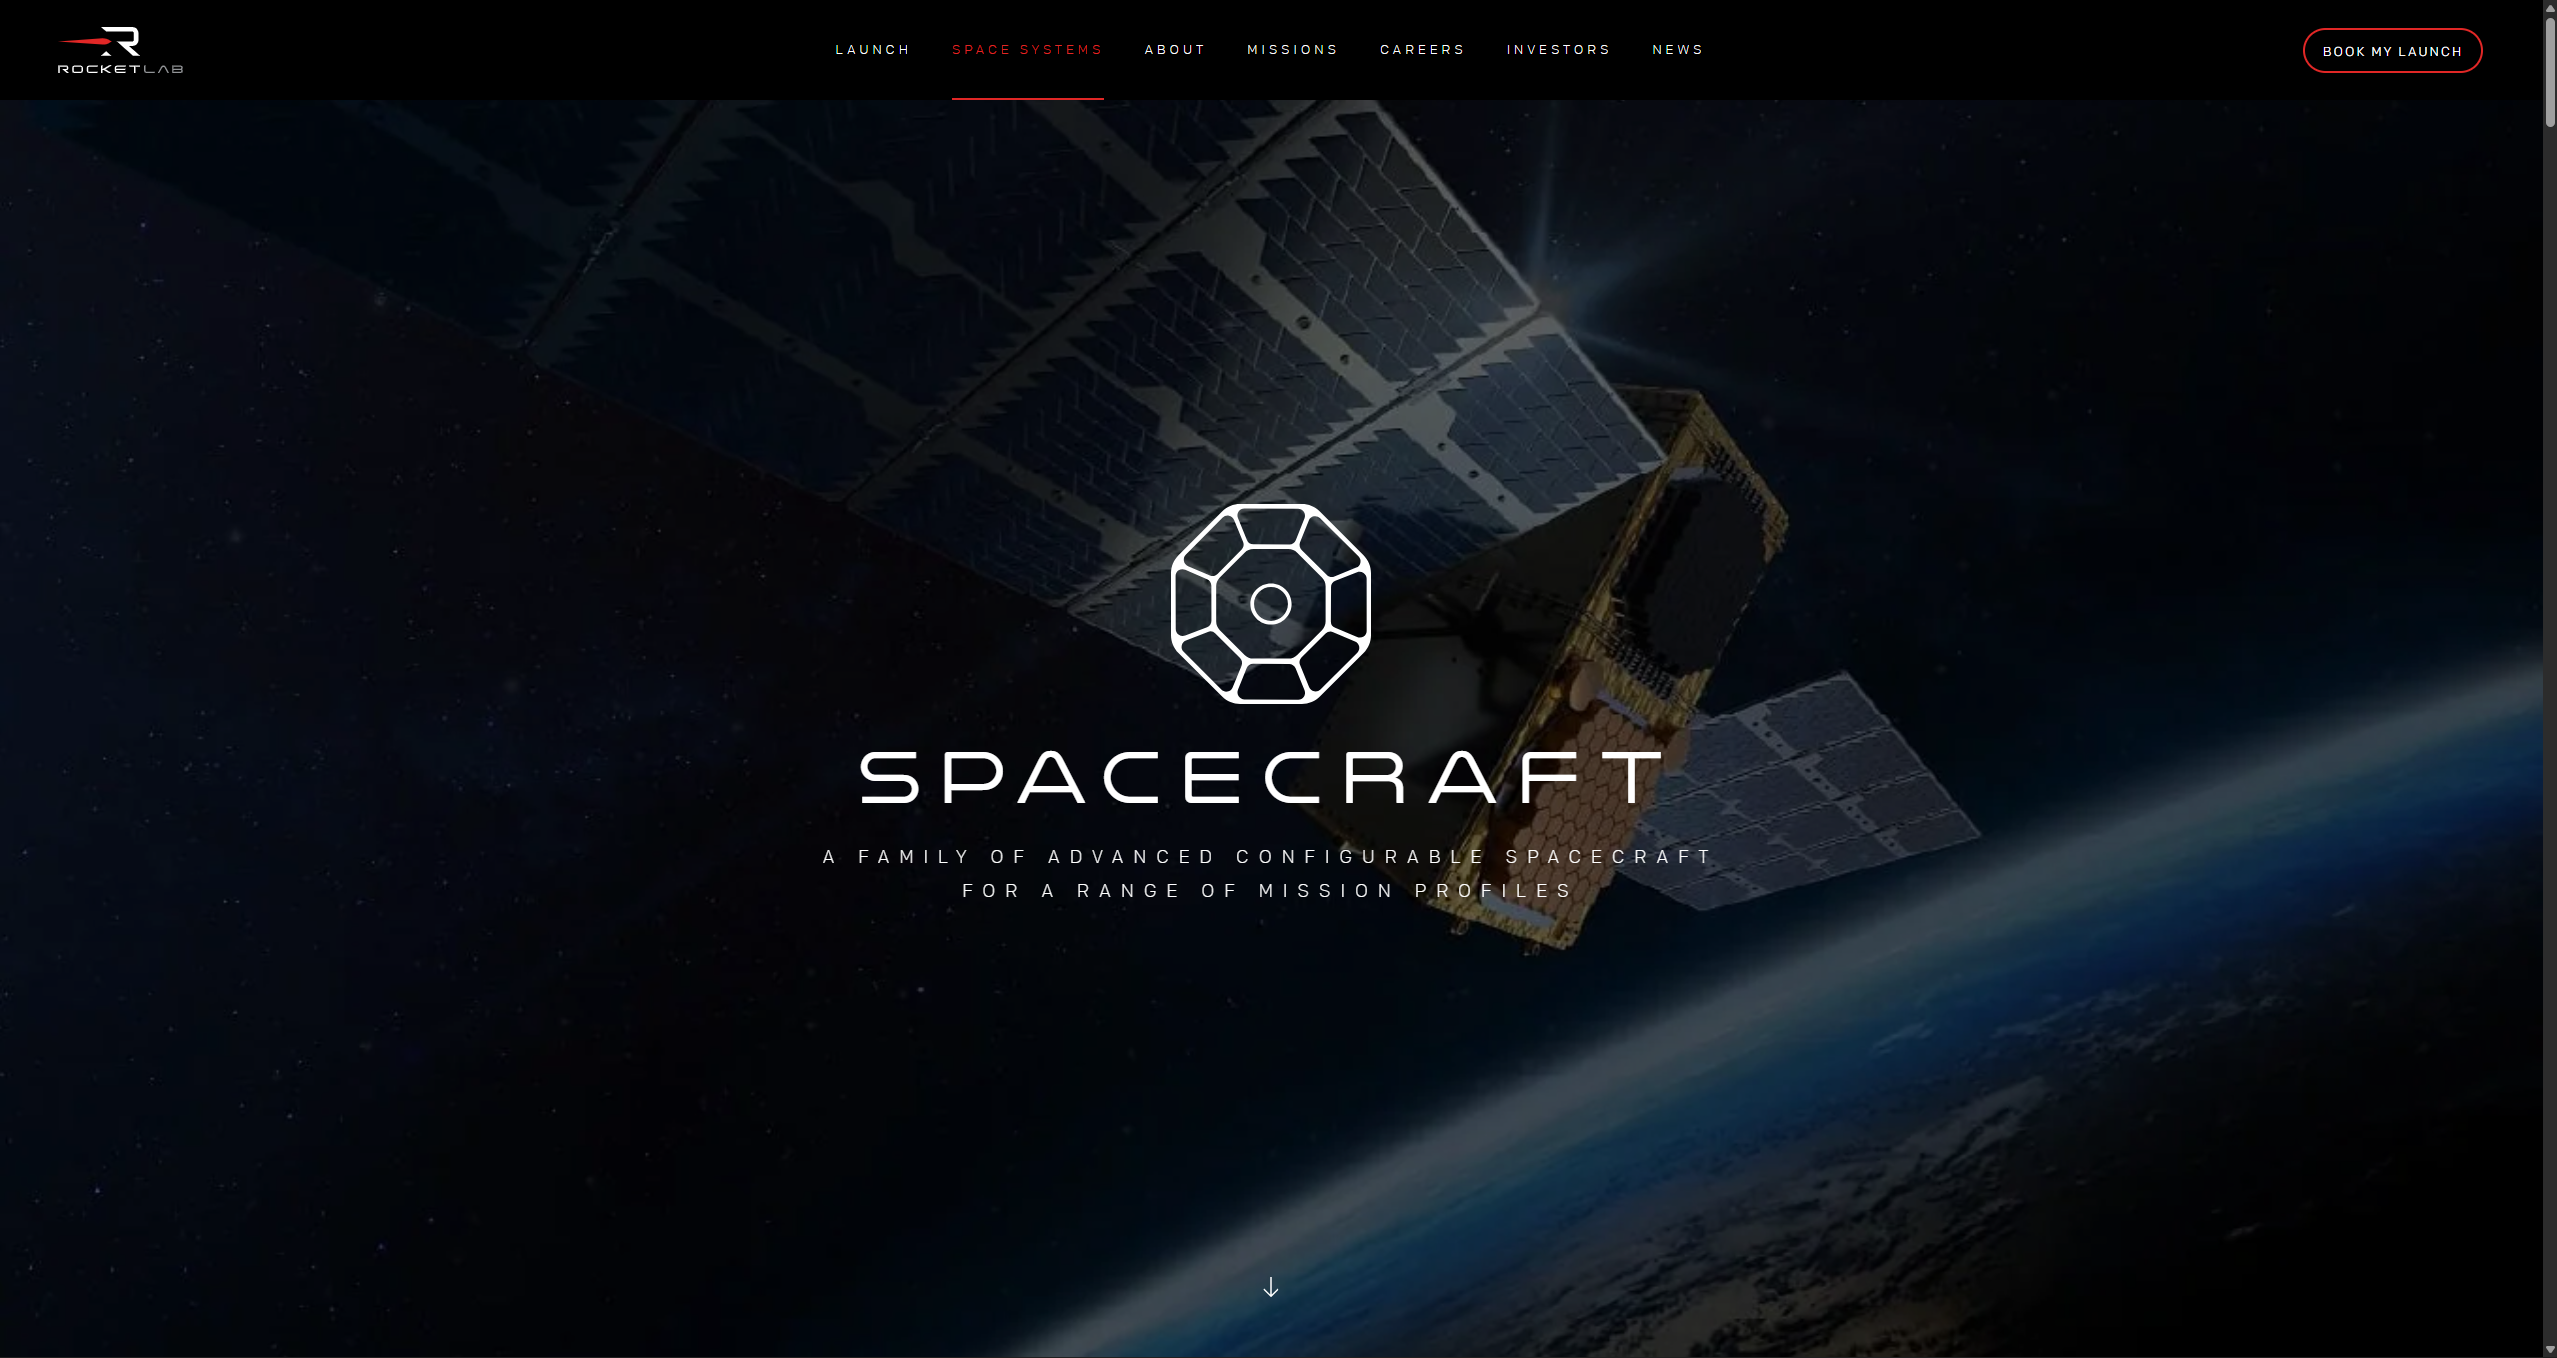
\includegraphics[width=1\linewidth]{SpaceCraft.png}
    \caption{Predstavitev spletne strani Rocket Lab \cite{rocketlab}.}
    \label{fig:rocketlab}
\end{figure}

\subsection{EnduroSat -- Space Service}

\textbf{Kratek opis:} \\
EnduroSat je evropsko vesoljsko podjetje, ki na svoji spletni platformi ponuja standardizirane satelitske platforme ter storitev gostovanja naročnikovega tovora v orbiti pod imenom Space Service \cite{endurosat}. Rešitev nagovarja podjetja, ki želijo svoje senzorje ali komunikacijsko opremo preizkusiti v vesolju brez razvoja lastnega satelita.

\textbf{Ključne funkcionalnosti:}
\begin{itemize}
    \item \textbf{Izbira aplikacijskega področja in razreda satelita:} Filtriranje ponudbe glede na namen misije ter prikaz platform razreda 200 kg in 500 kg.
    \item \textbf{Prikaz ključnih zmogljivosti in kazalnikov:} Pregled razpoložljive električne moči, hitrosti prenosa podatkov, življenjske dobe ter števila že izstreljenih satelitov.
    \item \textbf{Opis poteka misije in povpraševanje:} Korak za korakom prikazan proces od integracije tovora do upravljanja v orbiti prek oblačnega vmesnika skupaj z obrazcem za povpraševanje.
\end{itemize}

\textbf{Prednosti in slabosti:}
\begin{itemize}
    \item \textbf{Prednosti:} Zelo dobro pokriva model gostovanja tovora na skupni platformi, pregledno razčleni faze izvedbe misije in uporablja jasne številčne kazalnike zaupanja.
    \item \textbf{Slabosti:} Zaradi zelo obsežnega kataloga posameznih satelitskih komponent in modulov je stran za novega obiskovalca nekoliko nepregledna, natančnejše tehnične in cenovne podatke pa je mogoče pridobiti šele po oddaji povpraševanja.
\end{itemize}

\begin{figure}[H]
    \centering
    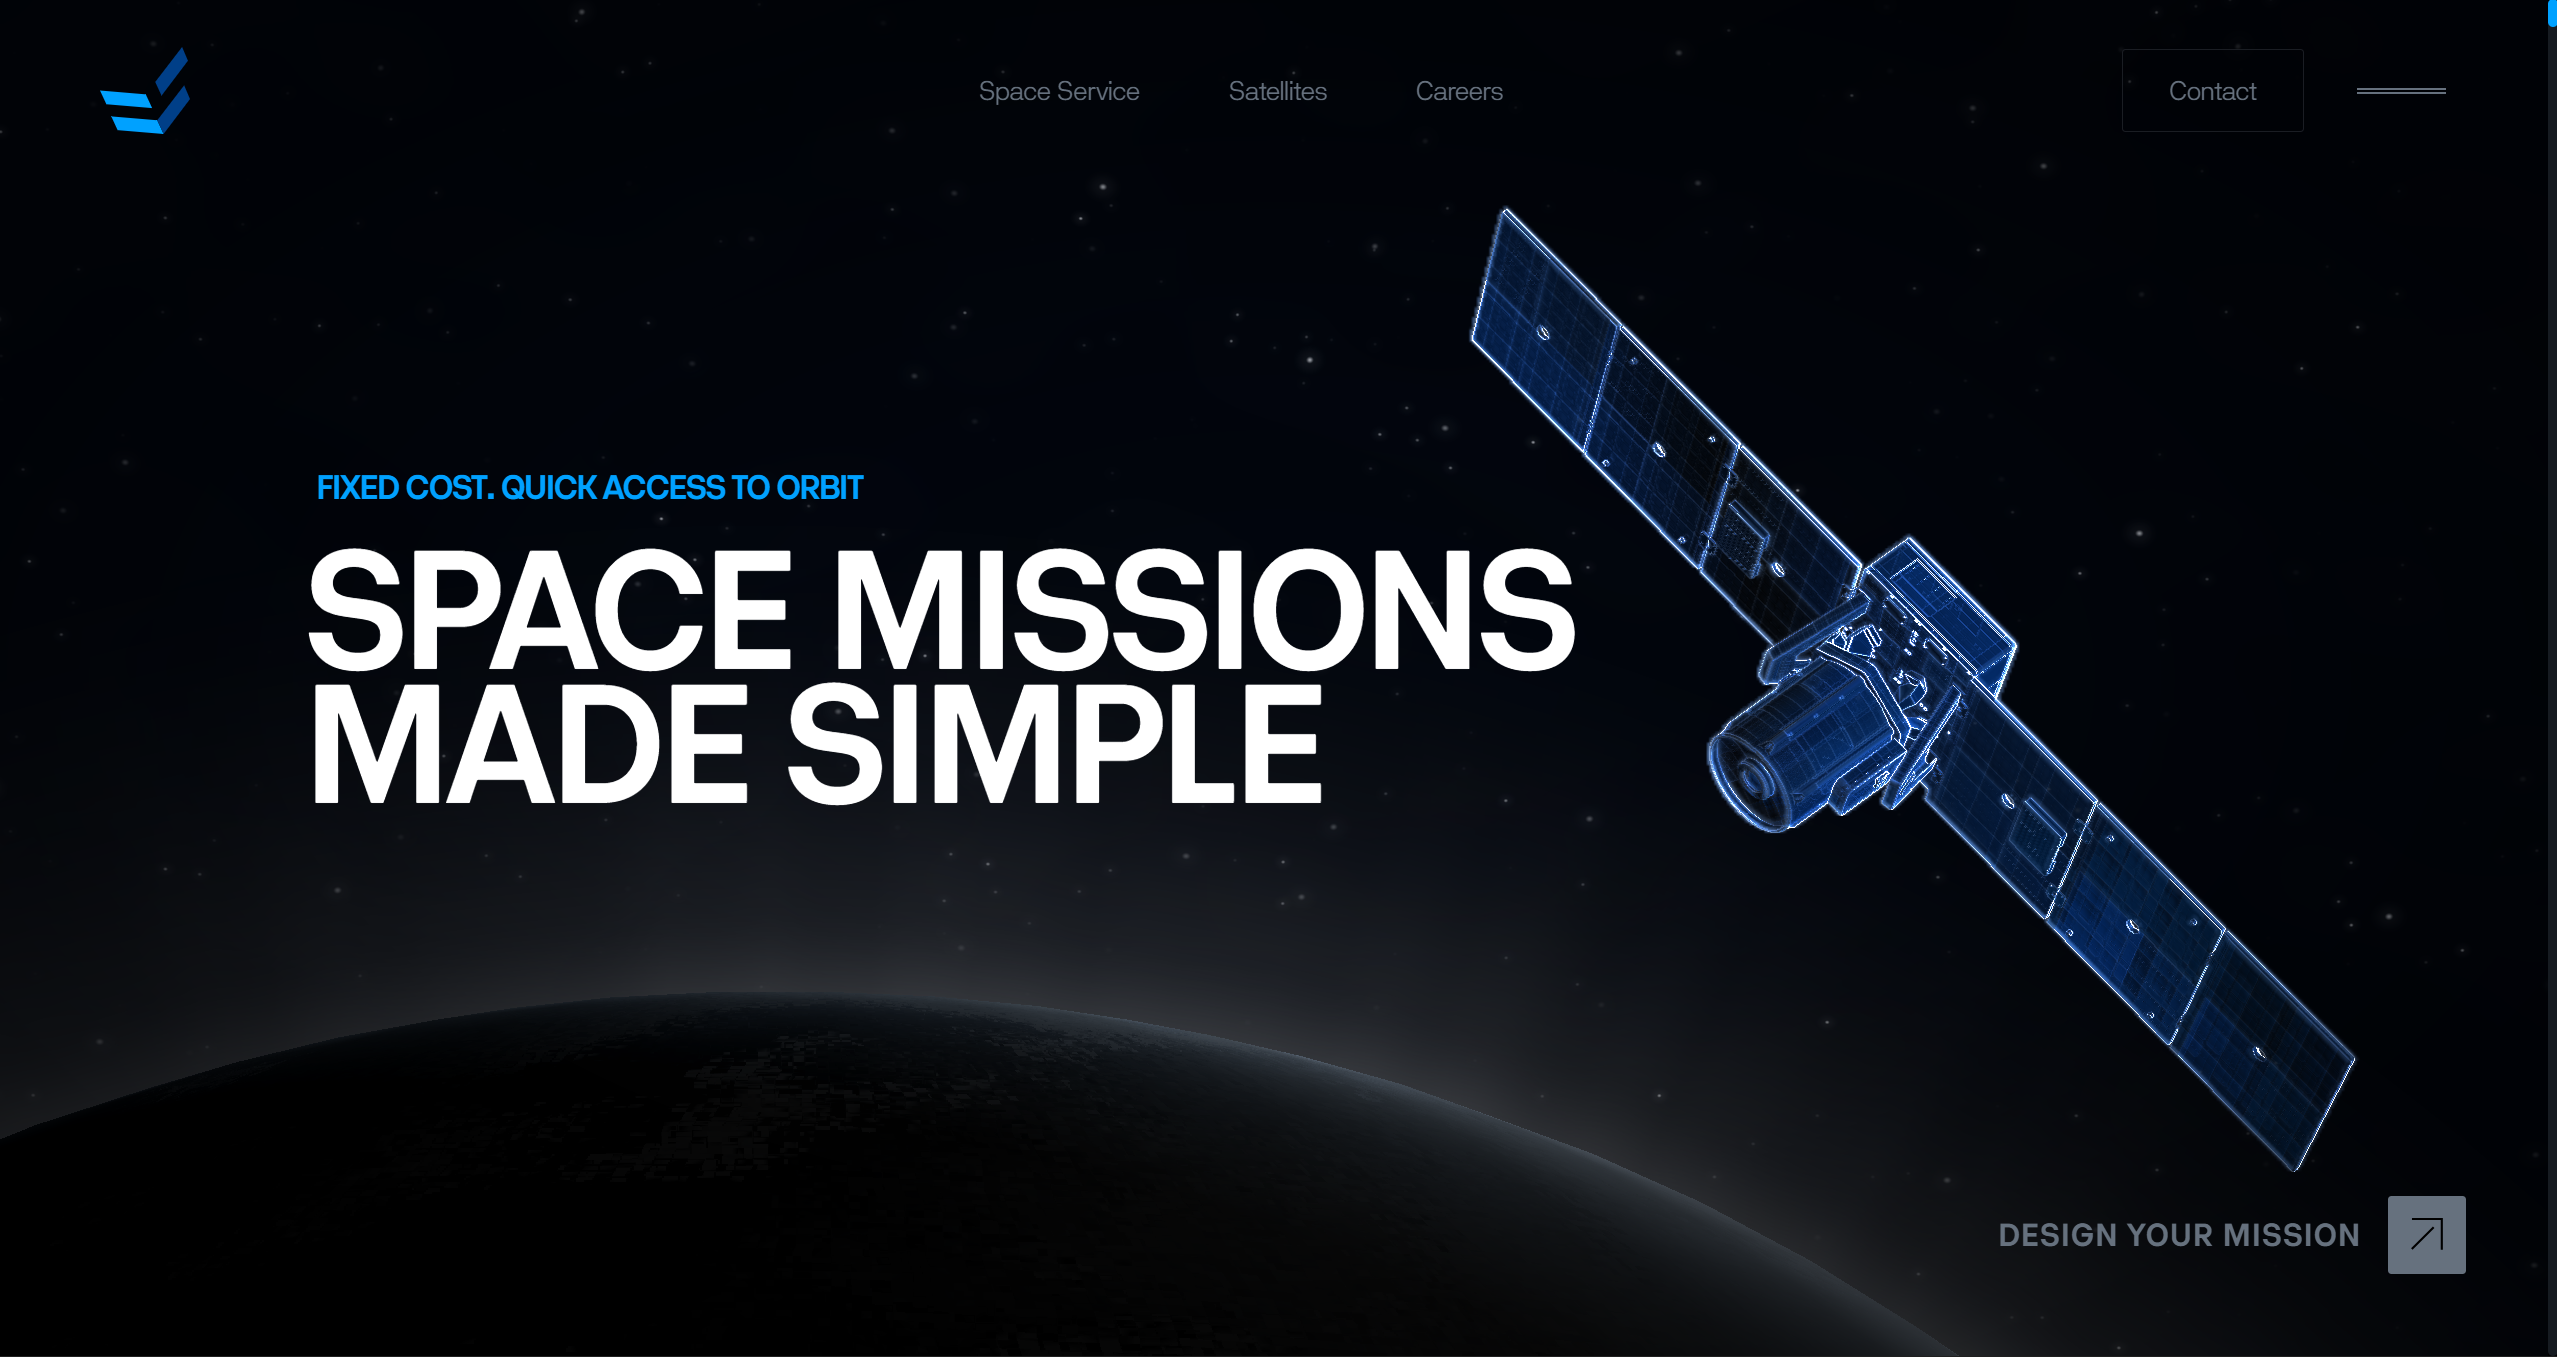
\includegraphics[width=1\linewidth]{EnduroSat.png}
    \caption{Spletna platforma EnduroSat \cite{endurosat}.}
    \label{fig:endurosat}
\end{figure}

\section{Zaključek}

Na podlagi pregleda vseh treh obstoječih rešitev smo prepoznali več dobrih praks, ki jih bomo vključili v razvoj spletne platforme \textbf{Nexus Orbital}:
\begin{itemize}
    \item \textbf{Temen, tehnično usmerjen vizualni slog in jasna hierarhija:} Po vzoru strani SpaceX Rideshare bomo uporabili pregledno razporeditev razdelkov z jasnimi poudarki na ključnih zmogljivostih in pozivih k dejanju.
    \item \textbf{Poudarek na tehnoloških stebrih in zaupanju partnerjev:} Podobno kot Rocket Lab in EnduroSat bomo že na začetku strani izpostavili ključne tehnologije podjetja.
\end{itemize}

Hkrati pa bo naša rešitev odpravila glavne pomanjkljivosti analiziranih spletnih mest in prinesla naslednje izboljšave:
\begin{itemize}
    \item \textbf{Takojšnje preklapljanje specifikacij flote brez osveževanja strani:} Namesto razpršenih podstrani in datotek PDF bo uporabnik v razdelku Fleet z enim klikom preklapljal med sateliti ter takoj primerjal maso, orbito, zmogljivost in življenjsko dobo.
    \item \textbf{Pregledna časovnica misij z oznakami stanja:} Na enem mestu bomo prikazali kronološki pregled misij z jasnimi oznakami statusa, kar obiskovalcu olajša oceno zrelosti tehnologije.
    \item \textbf{Poenostavljeno povpraševanje za tovor s takojšnjim preverjanjem vnosa:} V menuju kontaktno stran, kjer bomo ponudili kratek obrazec z takojšnjim preverjanjem obveznih polj in veljavnosti e-poštnega naslova ter neposrednimi podatki nadzornega centra.
\end{itemize}


\begin{table}[H]
    \centering
    \caption{Primerjava funkcionalnosti obstoječih rešitev in platforme Nexus Orbital.}
    \label{tab:primerjava}
    \makebox[\textwidth][c]{
        \begin{tabular}{lcccc}
            \toprule
            \textbf{Funkcionalnost} & \textbf{SpaceX Rideshare} & \textbf{Rocket Lab} & \textbf{EnduroSat} & \textbf{Nexus Orbital} \\
            \midrule
            Primerjava več satelitskih platform & Ne & Delno & Delno & \textbf{Da} \\
            Takojšnji prikaz specifikacij brez PDF & Delno & Ne & Ne & \textbf{Da} \\
            Časovnica misij z oznakami stanja & Ne & Delno & Ne & \textbf{Da} \\
            Obrazec za povpraševanje za tovor & Da & Da & Da & \textbf{Da} \\
            \bottomrule
        \end{tabular}
    }
\end{table}

\begin{thebibliography}{9}

\bibitem{spacex}
SpaceX, \emph{SmallSat Rideshare Program}, 2026. Dostopno na: \url{https://www.spacex.com/rideshare/} [pridobljeno 22. 11. 2026].

\bibitem{rocketlab}
Rocket Lab USA, \emph{Space Systems -- Spacecraft}, 2026. Dostopno na: \url{https://www.rocketlabusa.com/space-systems/spacecraft/} [pridobljeno 22. 11. 2026].

\bibitem{endurosat}
EnduroSat, \emph{Space Service -- Satellite Mission Design, Launch \& Operations}, 2026. Dostopno na: \url{https://www.endurosat.com/space-service/} [pridobljeno 22. 11. 2026].

\end{thebibliography}

\end{document}